%
% anwendungen.tex -- Anwendungen der elliptischen Funktionen
%
% (c) 2026 Baris Catan, OST Ostschweizer Fachhochschule
%
% !TEX root = ../../buch.tex
% !TEX encoding = UTF-8
%
\section{Anwendungen
\label{elliptisch:section:anwendungen}}
\kopfrechts{Anwendungen}

Mit dem Werkzeugkasten von
Abschnitt~\ref{elliptisch:subsection:werkzeugkasten} ist klar, woran
man eine jacobische Lösung erkennt.
Führt ein Problem auf die Differentialgleichung
\eqref{elliptisch:equation:signatur}, also das Quadrat der Ableitung
gleich einem Polynom vierten Grades, dann ist die Lösung eine
jacobische Funktion.
In diesem Abschnitt taucht diese Signatur dreimal auf.
Wir beginnen bei der Kurve, an der die Theorie historisch ihren
Anfang genommen hat, und kommen danach zu zwei physikalischen
Problemen, einem rotierenden Seil und einem Pendel.

\subsection{Die Lemniskate
\label{elliptisch:subsection:lemniskate}}
\index{Lemniskate}%
Die \emph{Lemniskate von Bernoulli} ist die Kurve vierten Grades
mit der Gleichung
\begin{equation}
(X^2+Y^2)^2 = 2a^2\,(X^2-Y^2).
\label{elliptisch:equation:lemniskate}
\end{equation}
Wir verwenden die Normierung $a = 1/\sqrt{2}$, in der die Scheitel
bei $(\pm 1, 0)$ liegen (Abbildung~\ref{fig:elliptisch:lemniskate}).
\input{papers/elliptisch/fig/lemniskateFIG.tex}%
In Polarkoordinaten schreibt sie sich als $r^2 = \cos 2\varphi$.
Das Bogenelement in Polarkoordinaten ist
$ds^2 = dr^2 + r^2\,d\varphi^2$, und Differenzieren der
Kurvengleichung ergibt $2r\,dr = -2\sin 2\varphi\,d\varphi$.
Damit lässt sich $\varphi$ eliminieren,
\begin{equation}
r^2\,d\varphi^2
=
\frac{r^4}{\sin^2 2\varphi}\,dr^2
=
\frac{r^4}{1-r^4}\,dr^2,
\end{equation}
denn es ist $\sin^2 2\varphi = 1 - \cos^2 2\varphi = 1 - r^4$.
Somit bleibt im Bogenelement nur noch der Radius,
\begin{equation}
ds
=
\sqrt{1 + \frac{r^4}{1-r^4}}\,dr
=
\frac{dr}{\sqrt{1-r^4}}.
\end{equation}
Die Bogenlänge vom Nullpunkt bis zum Punkt mit Radius $r$ ist damit
\begin{equation}
s(r)
=
\int_0^r \frac{dt}{\sqrt{1-t^4}}.
\label{elliptisch:equation:lemniskatebogen}
\end{equation}
Unter der Wurzel steht wieder ein Polynom vierten Grades, und der
Vergleich mit der Normalform in
\eqref{elliptisch:equation:normalformen} liefert
$(1-t^2)(1-k^2t^2) = 1-t^4$, also den Modul $k^2 = -1$.
Eine elementare Stammfunktion ist damit nicht zu erwarten, und der
Kontrast zum Kreis wiederholt sich.
Das Integral $\int_0^r dt/\sqrt{1-t^2} = \arcsin r$ bleibt
elementar, das Bogenlängenintegral der Lemniskate nicht.

Wie in \eqref{elliptisch:equation:umkehrung} kehren wir um.
Die Umkehrfunktion $r = \operatorname{sl}(s)$ heisst
\emph{lemniskatischer Sinus}.
\index{lemniskatischer Sinus}%
Der Bogen vom Nullpunkt bis zum Scheitel $(1,0)$ hat die Länge
$\varpi/2$, wobei
\begin{equation}
\varpi
=
2\int_0^1 \frac{dt}{\sqrt{1-t^4}}
=
2.6220575542\ldots
\label{elliptisch:equation:varpi}
\end{equation}
die Länge des rechten Blattes ist, die sogenannte
\emph{lemniskatische Konstante}.
\index{lemniskatische Konstante}%
Die Funktion $\operatorname{sl}$ ist $2\varpi$-periodisch, und was
für den Sinus die Zahl $\pi$ ist, ist für ihn $\varpi$.
Historisch war der lemniskatische Sinus die erste elliptische
Funktion überhaupt.
Gauss hat sie 1797 als Neunzehnjähriger in seinem mathematischen
Tagebuch untersucht, zu Lebzeiten aber nichts davon veröffentlicht
\cite{elliptisch:almkvist-berndt} und
\cite[Kapitel~11.3]{elliptisch:mueller-spezielle}.
Erst dreissig Jahre später wurde derselbe Umkehrschritt von Abel
und Jacobi in voller Allgemeinheit vollzogen
(Abschnitt~\ref{elliptisch:subsection:unvollstaendig}).

Die Verbindung zu den Jacobischen Funktionen gewinnt man aus der
Bogenlängenparametrisierung der Lemniskate.
Aus ihr folgt
\begin{equation}
\operatorname{sl}(s)
=
\operatorname{cn}\biggl(
\sqrt{2}\,\Bigl(\frac{\varpi}{2}-s\Bigr),\,
\frac{1}{\sqrt{2}}
\biggr),
\label{elliptisch:equation:sljacobi}
\end{equation}
der lemniskatische Sinus ist also bis auf Skalierung und
Verschiebung des Arguments die Funktion $\operatorname{cn}$ zum
Modul $k = 1/\sqrt{2}$
\cite[Kapitel~11.3]{elliptisch:mueller-spezielle}.
Insbesondere ist $\varpi = \sqrt{2}\,K(1/\sqrt{2})$, ganz analog zu
$\pi/2 = K(0)$ in \eqref{elliptisch:equation:randnull}.

\subsection{Das Troposkein
\label{elliptisch:subsection:troposkein}}
\index{Troposkein}%
\index{Springseil}%
Eine Schnur hängt zwischen zwei Punkten $A$ und $B$.
Unter der Schwerkraft nimmt sie die Kettenlinie an, einen
hyperbolischen Kosinus, ein durch und durch elementares Resultat.
Lassen wir dieselbe Schnur stattdessen mit der
Winkelgeschwindigkeit $\omega$ um die Verbindungsachse von $A$
und $B$ rotieren und vernachlässigen die Schwerkraft, entsteht
eine neue Gleichgewichtsform.
Sie heisst \emph{Troposkein} oder Springseilkurve
\cite{elliptisch:skipping-rope}.
Abbildung~\ref{fig:elliptisch:troposkein} zeigt das Profil der
rotierenden Schnur zwischen $A$ und $B$.
\begin{figure}
	\centering
	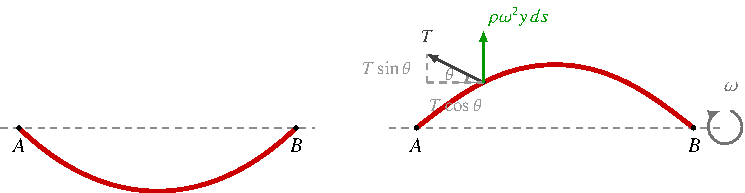
\includegraphics[width=\textwidth]{papers/elliptisch/images/troposkein.pdf}
	\caption{Links die hängende Schnur zwischen $A$ und $B$, die
	Kettenlinie $y(x) = a\cosh(x/a)$.
	Rechts dieselbe Schnur rotierend um die Achse $AB$, das
	Troposkein $y(x) = a\operatorname{sn}(x/c, k)$, mit der
	Zentrifugalkraft $\rho\omega^2y\,ds$ und der Seilspannung $T$ an
	einem Element bei Winkel $\theta$.}
	\label{fig:elliptisch:troposkein}
\end{figure}
%

Wir bezeichnen mit $y(x)$ den Abstand eines Seilpunktes von der
Drehachse, mit $\theta$ den Winkel der Seiltangente gegen die
Achse, mit $\rho$ die Linienmassendichte und mit $T$ die
Seilspannung (Abbildung~\ref{fig:elliptisch:troposkein}, rechts).
Auf ein Element der Länge $ds$ wirkt die Zentrifugalkraft
$\rho\omega^2 y\,ds$ radial nach aussen.
Im Gleichgewicht ist die axiale Komponente der Spannung konstant,
\begin{equation}
T\cos\theta = T_0,
\label{elliptisch:equation:troposkeinaxial}
\end{equation}
und die Änderung ihrer Querkomponente entlang der Bogenlänge trägt
die Zentrifugalkraft,
\begin{equation}
\frac{d(T\sin\theta)}{ds}
=
-\rho\omega^2 y.
\label{elliptisch:equation:troposkeinradial}
\end{equation}
Mit $T\sin\theta = T_0\tan\theta$ aus
\eqref{elliptisch:equation:troposkeinaxial} und
$dy/ds = \sin\theta$ lässt sich
\eqref{elliptisch:equation:troposkeinradial} integrieren und liefert
die Spannung als Funktion des Abstandes,
\begin{equation}
T(y)
=
T_0 + \frac{\rho\omega^2}{2}\,\bigl(a^2 - y^2\bigr),
\label{elliptisch:equation:troposkeinspannung}
\end{equation}
wobei $a$ der grösste Achsabstand ist, also der Scheitel der Kurve,
an dem $\theta = 0$ und $T = T_0$ gilt.
Die Spannung ist folglich in der Mitte am kleinsten und an den
Endpunkten am grössten.

Die Ableitung der Kurve ist $y' = \tan\theta$, und mit
$\tan^2\theta = (T/T_0)^2 - 1$ wird aus
\eqref{elliptisch:equation:troposkeinspannung} nach Quadrieren und
Zusammenfassen der Konstanten
\begin{equation}
(y')^2
=
\frac{1}{c^2}\,\bigl(a^2 - y^2\bigr)
\biggl(1 - \frac{b^2 y^2}{a^4}\biggr)
\label{elliptisch:equation:troposkein}
\end{equation}
mit zwei Konstanten $b \le a$ und $c$, die sich aus den
physikalischen Grössen und den Randbedingungen bestimmen.
Rechts steht ein Polynom vierten Grades in $y$, genau die Signatur
\eqref{elliptisch:equation:signatur} aus dem Werkzeugkasten.
Die Lösung muss daher eine jacobische Funktion sein.
Wir machen den Ansatz
\begin{equation}
y(x)
=
a\,\operatorname{sn}\Bigl(\frac{x}{c}, k\Bigr),
\qquad
k = \frac{b}{a},
\label{elliptisch:equation:troposkeinloesung}
\end{equation}
und setzen ihn zur Probe ein.
Nach \eqref{elliptisch:equation:sndgl} ist
$(y')^2 = (a^2/c^2)\,\operatorname{cn}^2\operatorname{dn}^2
= (1/c^2)\,(a^2-y^2)\,(1 - k^2y^2/a^2)$,
was mit $k = b/a$ genau die rechte Seite von
\eqref{elliptisch:equation:troposkein} ergibt.
Die Randbedingungen legen die Konstanten fest.
Das Seil geht bei $A$ und $B$ durch $y = 0$ und erreicht seine
grosste Auslenkung in der Mitte, also ist der Achsenabstand
$AB = 2c\,K(k)$, und die vorgegebene Seillänge liefert die zweite
Bedingung an $b$ und $c$.

Damit stellt sich heraus, dass das Auge uns hier täuscht.
Die Springseilkurve sieht aus wie eine Sinushalbwelle, ist aber
keine, erst recht keine Kettenlinie mehr, sondern ein Jacobischer
Sinus als Funktion des \emph{Ortes}.
Dieselbe Gleichung \eqref{elliptisch:equation:troposkein} wird uns
in Abschnitt~\ref{elliptisch:subsection:pendel} wieder begegnen,
dort mit der Zeit als unabhängiger Variable.
Die Form hat auch eine technische Seite.
Die Schaufeln des Darrieus-Rotors werden im Troposkein-Profil
gebaut, weil die Zentrifugalkraft ein Seil in dieser Form nur auf
Zug belastet und nicht auf Biegung
\cite{elliptisch:wiki-darrieus}.
\index{Darrieus-Rotor}%

\subsection{Das Pendel
\label{elliptisch:subsection:pendel}}
